\documentclass{article}[12pt]

\addtolength{\oddsidemargin}{-.75in}%
\addtolength{\evensidemargin}{-.75in}%
\addtolength{\textwidth}{1.5in}%
\addtolength{\textheight}{1.3in}%
\addtolength{\topmargin}{-.8in}%
\addtolength{\marginparpush}{-.75in}%
%\setlength\parindent{0pt}
%\setlength{\bibsep}{0pt plus 0.3ex}

\usepackage[authoryear]{natbib}
\usepackage{graphicx}
\usepackage{algorithm,algorithmic}

\title{Variational approximations to zero-inflated Bayesian models}
\author{Mark Greenaway}
% include.tex
\newcommand{\Bernoulli}[1]{\text{Bernoulli} \left( #1 \right)}
\newcommand{\mydigamma}[1]{\psi \left( #1 \right)}
%\newcommand{\diag}[1]{\text{diag}\left( #1 \right)}
\newcommand{\tr}[1]{\text{tr}\left( #1 \right)}
\newcommand{\Poisson}[1]{\text{Poisson} \left( #1 \right)}
\def \half {\frac{1}{2}}
\def \R {\mathbb{R}}
\def \vbeta {\vec{\beta}}
\def \vy {\vec{y}}
\def \vmu {\vec{\mu}}
\def \vmuqbeta {\vmu_{q(\vbeta)}}
\def \vmubeta {\vmu_{\vbeta}}
\def \Sigmaqbeta {\Sigma_{q(\vbeta)}}
\def \Sigmabeta {\Sigma_{\vbeta}}
\def \va {\vec{a}}
\def \vtheta {\vec{\theta}}
\def \mX {\vec{X}}

\def\ds{{\displaystyle}}

\def\diag{{\mbox{diag}}}


\usepackage{latexsym,amssymb,amsmath,amsfonts}
%\usepackage{tabularx}
\usepackage{theorem}
\usepackage{verbatim,array,multicol,palatino}
\usepackage{graphicx}
\usepackage{graphics}
\usepackage{fancyhdr}
\usepackage{algorithm,algorithmic}
\usepackage{url}
%\usepackage[all]{xy}



\def\approxdist{\stackrel{{\tiny \mbox{approx.}}}{\sim}}
\def\smhalf{\textstyle{\frac{1}{2}}}
\def\vxnew{\vx_{\mbox{{\tiny new}}}}
\def\bib{\vskip12pt\par\noindent\hangindent=1 true cm\hangafter=1}
\def\jump{\vskip3mm\noindent}
\def\etal{{\em et al.}}
\def\etahat{{\widehat\eta}}
\def\thick#1{\hbox{\rlap{$#1$}\kern0.25pt\rlap{$#1$}\kern0.25pt$#1$}}
\def\smbbeta{{\thick{\scriptstyle{\beta}}}}
\def\smbtheta{{\thick{\scriptstyle{\theta}}}}
\def\smbu{{\thick{\scriptstyle{\rm u}}}}
\def\smbzero{{\thick{\scriptstyle{0}}}}
\def\boxit#1{\begin{center}\fbox{#1}\end{center}}
\def\lboxit#1{\vbox{\hrule\hbox{\vrule\kern6pt
      \vbox{\kern6pt#1\kern6pt}\kern6pt\vrule}\hrule}}
\def\thickboxit#1{\vbox{{\hrule height 1mm}\hbox{{\vrule width 1mm}\kern6pt
          \vbox{\kern6pt#1\kern6pt}\kern6pt{\vrule width 1mm}}
               {\hrule height 1mm}}}


%\sloppy
%\usepackage{geometry}
%\geometry{verbose,a4paper,tmargin=20mm,bmargin=20mm,lmargin=40mm,rmargin=20mm}


%%%%%%%%%%%%%%%%%%%%%%%%%%%%%%%%%%%%%%%%%%%%%%%%%%%%%%%%%%%%%%%%%%%%%%%%%%%%%%%%
%
% Some convenience definitions
%
% \bf      -> vector
% \sf      -> matrix
% \mathcal -> sets or statistical
% \mathbb  -> fields or statistical
%
%%%%%%%%%%%%%%%%%%%%%%%%%%%%%%%%%%%%%%%%%%%%%%%%%%%%%%%%%%%%%%%%%%%%%%%%%%%%%%%%

% Sets or statistical values
\def\sI{{\mathcal I}}                            % Current Index set
\def\sJ{{\mathcal J}}                            % Select Index set
\def\sL{{\mathcal L}}                            % Likelihood
\def\sl{{\ell}}                                  % Log-likelihood
\def\sN{{\mathcal N}}                            
\def\sS{{\mathcal S}}                            
\def\sP{{\mathcal P}}                            
\def\sQ{{\mathcal Q}}                            
\def\sB{{\mathcal B}}                            
\def\sD{{\mathcal D}}                            
\def\sT{{\mathcal T}}
\def\sE{{\mathcal E}}                            
\def\sF{{\mathcal F}}                            
\def\sC{{\mathcal C}}                            
\def\sO{{\mathcal O}}                            
\def\sH{{\mathcal H}} 
\def\sR{{\mathcal R}}                            
\def\sJ{{\mathcal J}}                            
\def\sCP{{\mathcal CP}}                            
\def\sX{{\mathcal X}}                            
\def\sA{{\mathcal A}} 
\def\sZ{{\mathcal Z}}                            
\def\sM{{\mathcal M}}                            
\def\sK{{\mathcal K}}     
\def\sG{{\mathcal G}}                         
\def\sY{{\mathcal Y}}                         
\def\sU{{\mathcal U}}  


\def\sIG{{\mathcal IG}}                            


\def\cD{{\sf D}}
\def\cH{{\sf H}}
\def\cI{{\sf I}}

% Vectors
\def\vectorfontone{\bf}
\def\vectorfonttwo{\boldsymbol}
\def\va{{\vectorfontone a}}                      %
\def\vb{{\vectorfontone b}}                      %
\def\vc{{\vectorfontone c}}                      %
\def\vd{{\vectorfontone d}}                      %
\def\ve{{\vectorfontone e}}                      %
\def\vf{{\vectorfontone f}}                      %
\def\vg{{\vectorfontone g}}                      %
\def\vh{{\vectorfontone h}}                      %
\def\vi{{\vectorfontone i}}                      %
\def\vj{{\vectorfontone j}}                      %
\def\vk{{\vectorfontone k}}                      %
\def\vl{{\vectorfontone l}}                      %
\def\vm{{\vectorfontone m}}                      % number of basis functions
\def\vn{{\vectorfontone n}}                      % number of training samples
\def\vo{{\vectorfontone o}}                      %
\def\vp{{\vectorfontone p}}                      % number of unpenalized coefficients
\def\vq{{\vectorfontone q}}                      % number of penalized coefficients
\def\vr{{\vectorfontone r}}                      %
\def\vs{{\vectorfontone s}}                      %
\def\vt{{\vectorfontone t}}                      %
\def\vu{{\vectorfontone u}}                      % Penalized coefficients
\def\vv{{\vectorfontone v}}                      %
\def\vw{{\vectorfontone w}}                      %
\def\vx{{\vectorfontone x}}                      % Covariates/Predictors
\def\vy{{\vectorfontone y}}                      % Targets/Labels
\def\vz{{\vectorfontone z}}                      %

\def\vone{{\vectorfontone 1}}
\def\vzero{{\vectorfontone 0}}

\def\valpha{{\vectorfonttwo \alpha}}             %
\def\vbeta{{\vectorfonttwo \beta}}               % Unpenalized coefficients
\def\vgamma{{\vectorfonttwo \gamma}}             %
\def\vdelta{{\vectorfonttwo \delta}}             %
\def\vepsilon{{\vectorfonttwo \epsilon}}         %
\def\vvarepsilon{{\vectorfonttwo \varepsilon}}   % Vector of errors
\def\vzeta{{\vectorfonttwo \zeta}}               %
\def\veta{{\vectorfonttwo \eta}}                 % Vector of natural parameters
\def\vtheta{{\vectorfonttwo \theta}}             % Vector of combined coefficients
\def\vvartheta{{\vectorfonttwo \vartheta}}       %
\def\viota{{\vectorfonttwo \iota}}               %
\def\vkappa{{\vectorfonttwo \kappa}}             %
\def\vlambda{{\vectorfonttwo \lambda}}           % Vector of smoothing parameters
\def\vmu{{\vectorfonttwo \mu}}                   % Vector of means
\def\vnu{{\vectorfonttwo \nu}}                   %
\def\vxi{{\vectorfonttwo \xi}}                   %
\def\vpi{{\vectorfonttwo \pi}}                   %
\def\vvarpi{{\vectorfonttwo \varpi}}             %
\def\vrho{{\vectorfonttwo \rho}}                 %
\def\vvarrho{{\vectorfonttwo \varrho}}           %
\def\vsigma{{\vectorfonttwo \sigma}}             %
\def\vvarsigma{{\vectorfonttwo \varsigma}}       %
\def\vtau{{\vectorfonttwo \tau}}                 %
\def\vupsilon{{\vectorfonttwo \upsilon}}         %
\def\vphi{{\vectorfonttwo \phi}}                 %
\def\vvarphi{{\vectorfonttwo \varphi}}           %
\def\vchi{{\vectorfonttwo \chi}}                 %
\def\vpsi{{\vectorfonttwo \psi}}                 %
\def\vomega{{\vectorfonttwo \omega}}             %


% Matrices
%\def\matrixfontone{\sf}
%\def\matrixfonttwo{\sf}
\def\matrixfontone{\bf}
\def\matrixfonttwo{\boldsymbol}
\def\mA{{\matrixfontone A}}                      %
\def\mB{{\matrixfontone B}}                      %
\def\mC{{\matrixfontone C}}                      % Combined Design Matrix
\def\mD{{\matrixfontone D}}                      % Penalty Matrix for \vu_J
\def\mE{{\matrixfontone E}}                      %
\def\mF{{\matrixfontone F}}                      %
\def\mG{{\matrixfontone G}}                      % Penalty Matrix for \vu
\def\mH{{\matrixfontone H}}                      %
\def\mI{{\matrixfontone I}}                      % Identity Matrix
\def\mJ{{\matrixfontone J}}                      %
\def\mK{{\matrixfontone K}}                      %
\def\mL{{\matrixfontone L}}                      % Lower bound
\def\mM{{\matrixfontone M}}                      %
\def\mN{{\matrixfontone N}}                      %
\def\mO{{\matrixfontone O}}                      %
\def\mP{{\matrixfontone P}}                      %
\def\mQ{{\matrixfontone Q}}                      %
\def\mR{{\matrixfontone R}}                      %
\def\mS{{\matrixfontone S}}                      %
\def\mT{{\matrixfontone T}}                      %
\def\mU{{\matrixfontone U}}                      % Upper bound
\def\mV{{\matrixfontone V}}                      %
\def\mW{{\matrixfontone W}}                      % Variance Matrix i.e. diag(b'')
\def\mX{{\matrixfontone X}}                      % Unpenalized Design Matrix/Nullspace Matrix
\def\mY{{\matrixfontone Y}}                      %
\def\mZ{{\matrixfontone Z}}                      % Penalized Design Matrix/Kernel Space Matrix

\def\mGamma{{\matrixfonttwo \Gamma}}             %
\def\mDelta{{\matrixfonttwo \Delta}}             %
\def\mTheta{{\matrixfonttwo \Theta}}             %
\def\mLambda{{\matrixfonttwo \Lambda}}           % Penalty Matrix for \vnu
\def\mXi{{\matrixfonttwo \Xi}}                   %
\def\mPi{{\matrixfonttwo \Pi}}                   %
\def\mSigma{{\matrixfonttwo \Sigma}}             %
\def\mUpsilon{{\matrixfonttwo \Upsilon}}         %
\def\mPhi{{\matrixfonttwo \Phi}}                 %
\def\mOmega{{\matrixfonttwo \Omega}}             %
\def\mPsi{{\matrixfonttwo \Psi}}                 %

\def\mone{{\matrixfontone 1}}
\def\mzero{{\matrixfontone 0}}

% Fields or Statistical
\def\bE{{\mathbb E}}                             % Expectation
\def\bP{{\mathbb P}}                             % Probability
\def\bR{{\mathbb R}}                             % Reals
\def\bI{{\mathbb I}}                             % Reals
\def\bV{{\mathbb V}}                             % Reals

\def\vX{{\vectorfontone X}}                      % Targets/Labels
\def\vY{{\vectorfontone Y}}                      % Targets/Labels
\def\vZ{{\vectorfontone Z}}                      %

% Other
\def\etal{{\em et al.}}
\def\ds{\displaystyle}
\def\d{\partial}
\def\diag{\text{diag}}
%\def\span{\text{span}}
\def\blockdiag{\text{blockdiag}}
\def\tr{\text{tr}}
\def\RSS{\text{RSS}}
\def\df{\text{df}}
\def\GCV{\text{GCV}}
\def\AIC{\text{AIC}}
\def\MLC{\text{MLC}}
\def\mAIC{\text{mAIC}}
\def\cAIC{\text{cAIC}}
\def\rank{\text{rank}}
\def\MASE{\text{MASE}}
\def\SMSE{\text{SASE}}
\def\sign{\text{sign}}
\def\card{\text{card}}
\def\notexp{\text{notexp}}
\def\ASE{\text{ASE}}
\def\ML{\text{ML}}
\def\nullity{\text{nullity}}

\def\logexpit{\text{logexpit}}
\def\logit{\mbox{logit}}
\def\dg{\mbox{dg}}

\def\Bern{\mbox{Bernoulli}}
\def\sBernoulli{\mbox{Bernoulli}}
\def\sGamma{\mbox{Gamma}}
\def\sInvN{\mbox{Inv}\sN}
\def\sNegBin{\sN\sB}

\def\dGamma{\mbox{Gamma}}
\def\dInvGam{\mbox{Inv}\Gamma}

\def\Cov{\mbox{Cov}}
\def\Mgf{\mbox{Mgf}}

\def\mis{{mis}} 
\def\obs{{obs}}

\def\argmax{\operatornamewithlimits{\text{argmax}}}
\def\argmin{\operatornamewithlimits{\text{argmin}}}
\def\argsup{\operatornamewithlimits{\text{argsup}}}
\def\arginf{\operatornamewithlimits{\text{arginf}}}


\def\minimize{\operatornamewithlimits{\text{minimize}}}
\def\maximize{\operatornamewithlimits{\text{maximize}}}
\def\suchthat{\text{such that}}


\def\relstack#1#2{\mathop{#1}\limits_{#2}}
\def\sfrac#1#2{{\textstyle{\frac{#1}{#2}}}}


\def\comment#1{
\vspace{0.5cm}
\noindent \begin{tabular}{|p{14cm}|}  
\hline #1 \\ 
\hline 
\end{tabular}
\vspace{0.5cm}
}


\def\mytext#1{\begin{tabular}{p{13cm}}#1\end{tabular}}
\def\mytextB#1{\begin{tabular}{p{7.5cm}}#1\end{tabular}}
\def\mytextC#1{\begin{tabular}{p{12cm}}#1\end{tabular}}

\def\jump{\vskip3mm\noindent}

\def\KL{\text{KL}}
\def\N{\text{N}}
\def\Var{\text{Var}}

\def \E {\mathbb{E}}
\def \BigO {\text{O}}
\def \IG {\text{IG}}
\def \Beta {\text{Beta}}


\begin{document}
\maketitle

Abstract:

Keywords: Approximate Bayesian inference . mixed model . Markov chain Monte Carlo

\section{Introduction}

% First, simplest zero-inflated count model to consider.
\noindent Count data with a large number of zero counts arises in many areas of
application, such as data arising from physical activity studies, 
insurance claims, hospital visits or defects in manufacturing processes.

While simple forms of these models are easy to fit with maximum likelihood techniques,
more general models incorporating random effects, splines and missing data typically
have no closed form solutions. Fitting these models is typically done with Monte Carlo
Markov Chain techniques, but these can be slow and prone to convergence problems. We
propose to use Variational Bayes to fit close approximations to these models
using a deterministic algorithm which converges much more quickly.

% Cite prior publications in this area

In this paper, we follow the earlier work of \ldots

In Section \ref{sec:methodology} we provide the framework for our approach. In
Section \ref{sec:methodology} we extend our approach to incorporate regression modelling
and random effects. In Section \ref{sec:results} we show how our approach offers 
computational advantages over existing approaches. In Section \ref{sec:application} we 
show an application of our method to physical activity data. Appendices contain details 
of our MCMC samplers.

\subsection{Notation}

The notation $\vx \sim N(\vmu, \mSigma)$ means that $\vx$ has a multivariate normal
density with mean $\vmu$ and covariance $\mSigma$. If $x$ has an inverse gamma
distribution, denoted $x \sim \mbox{IG}(\alpha, \beta)$, then it has density
$p(x) = \beta^\alpha \Gamma(\alpha)^{-1}x^{-\alpha-1} \exp{(-\beta/x)}, x, \alpha,
\beta > 0$.
If $\vx$ is a vector of length $d$ then $\mbox{diag}(\vx)$ is the $d \times d$
diagonal matrix whose diagonal elements are $\vx$.

\section{Methodology}\label{sec:methodology}

In this section we present a VB approach to a Bayesian zero-inflated Poisson model
for count data with extra zeroes. After introducing Bayesian zero-inflated models
and VB methodology we derive the VB factorised approximation to the full Bayesian
model. 

\subsection{Variational Bayesian inference}

\subsection{Variational Bayes for zero-inflated count models}

\noindent We start with the simplest example of a zero-inflated Poisson model. Let

$$
y_i = r_i x_i, 1 \leq i \leq n,
$$

\noindent where $x_i \sim \Poisson{(\lambda)}$ independent of $r_i \stackrel{\text{ind.}}{\sim} \Bernoulli{(\rho)}, 1 \leq i \leq n$. We use vague priors
$\rho \sim \Unif{(0, 1)}$ and $\lambda \sim \myGamma{(0.01, 0.01)}$. 

 
% TODO: Add graphical model

  We use a factorised approximation to the full likelihood, as detailed in \citep{ormerod10}.
The use of conjugate priors in the full model yields easier mean field updates in the
variational approximation.

  It can be shown via standard algebraic manipulations that the
full conditionals for $\lambda, \rho$ and $\vr$ are:

$$
\begin{array}{rl}
\lambda | \textbf{rest} &\sim \myGamma{(\alpha_\lambda + \vone^T\vx, \beta_\lambda + \vone^T\vr)}, \\ [0.5ex]
\rho | \textbf{rest} &\sim \Beta{(\alpha_\rho + \vone^T \vr, \beta_\rho + n - \vone^T\vr)} \\ [0.5ex]
\mbox{ and } \quad r_i | \textbf{rest} &\sim \Bernoulli{(\text{expit}(\eta_i))}, \quad 1 \leq i \leq n.
\end{array}
$$

% Step Two: Assume q(r_i) = Bernoulli(\rho_i), 1 \leq i \leq n for some known \rho_i. Find the
% variational Bayes updates of the q-densities q(\lambda) and q(\rho) corresponding to the
% factorisation
% q(\vr, \lambda, \rho) = q(\lambda) q(\rho) \sum_{i=1}^n q(r_i)

\noindent We assume a factorised approximation of the form

$$
q(\lambda, \rho, \vp) = q(\lambda) q(\rho) \left [ \prod_{i=1}^n q(r_i) \right ]
$$

\noindent where $q(\lambda)$ is a Gamma distribution, $q(\rho)$ is a Beta distribution and
$q(r_i)$ are Bernoulli distributions.

\noindent This leads to the following functional forms of the optimal q-densities

$$
\begin{array}{l}
\mbox{$q^*(\lambda)$ is the $\myGamma{\alpha_{q(\lambda)}, \beta_{q(\lambda)}}$ density function,} \\ [0.5ex]
\mbox{$q^*(\rho)$ is the $\text{Beta}(\alpha_{q(\rho)}, \beta_{q(\rho)})$ density function, and} \\ [0.5ex]
\mbox{$q^*(r_i)$  is the $\text{Bernoulli}(p_{q(r_i)})$ density function, $1 \leq i \leq n$,}
\end{array}
$$

%$$
%\begin{array}{c}
%q^*(\lambda) \sim \myGamma(\alpha_{q(\lambda)}, %\beta_{q(\lambda)}),
%q^*(\rho) \sim \text{Beta}(\alpha_{q(\rho)}, \beta_{q(\rho)}),
%\quad \mbox{ and } \quad  
%q^*(r_i) \sim \text{Bernoulli}(p_{q(r_i)}), \ \ 1 \leq i \leq n,
%\end{array}
%$$

\noindent where the parameters are updated according to Algorithm \ref{algorithm1}. 

\subsection{Lower bound}
The lower bound of the univariate model can be calculated directly to be
$$
\begin{array}{rl}
\bE_q \left\{ \log{p(\vx, \vr, \lambda, \rho)} - \log{q(\vr, \lambda, \rho)} \right\} &= T_1 + T_2 \\
\end{array}
$$

\noindent where
$$
\begin{array}{rl}
T_1 & \ds =
\alpha_\lambda \log{(\beta_\lambda)} + (\alpha_\lambda - 1) [\psi(\alpha_{q(\lambda)}) - \log{(\beta_{q(\lambda)})}] - \beta_\lambda \frac{\alpha_{q(\lambda)}}{\beta_{q(\lambda)}} - \log\Gamma(\alpha_\lambda) \\
& \ds \quad -\vp^T\frac{\alpha_{q(\lambda)}}{\beta_{q(\lambda)}} + \bE_q[\vx^T \log{(\lambda \vr)}] - \log\Gamma(\vx+1)) \quad \mbox{and} 
\\ [1ex]
T_2 &= \quad \left [ \sum_{i \in 0} - p_i \log p_i - (1 - p_i) \log (1 - p_i) \right ] \\
& \quad - \log \Beta (\alpha_\rho, \beta_\rho) + \log \Beta (\alpha_q, \beta_q)
\end{array}
$$

\noindent with 
$$
\bE [x_i \log{(\lambda r_i)}]  =
	\begin{cases}
	0 & \textbf{if } x_i = 0 \\
	\bE_q [\log \lambda] = \psi(\alpha_{q(\lambda)}) - \log{(\beta_{q(\lambda)})} & \textbf{if } x_i \ne 0. \\
	\end{cases}
$$

\begin{algorithm} 
\caption[Algorithm 1]{Iterative scheme for obtaining the parameters in the
optimal densities $q^*(\lambda)$ and $q^*(\rho)$}
\begin{algorithmic}
\REQUIRE{$\alpha_{q(\rho)} \leftarrow \alpha_\rho + \vone^T\vp, 
\alpha_{q(\lambda)} \leftarrow \alpha_\lambda + \vone^T\vx$}
\WHILE{the increase in $\log{\underline{p}}(\vx;q)$ is significant}
\STATE $\beta_{q(\rho)} \leftarrow \beta_\rho + n - \vone^T\vp$
\STATE $\eta \leftarrow -\alpha_{q(\lambda)}/\beta_{q(\lambda)} + \psi{(a_{q{(\rho)}})} - \psi{(b_{q{(\rho)}})}$
\STATE $\vp_{q(\vr_0)} \leftarrow \expit{(\eta)}$
\STATE $\beta_{q(\lambda)} \leftarrow \beta_\lambda + \vone^T\vp$
\ENDWHILE
\end{algorithmic}
\label{algorithm1}
\end{algorithm}

%By taking the expectation of each full conditional with respect to 

% This should be made the numerical experiment section.
\subsection{Results}
A data set of 10,000 points were simulated from the univariate ZIP model with
$\lambda = 1$ and $\rho = 0.5$. The vague gamma prior $\alpha_\lambda = 0.01$ and $\beta_\lambda = 0.01$ was chosen for $\lambda$.

The convergence of the lower bound of the model is shown in Figure 
\ref{fig:univariate_lower_bound}.

\begin{figure}
\caption{Convergence of the univariate lower bound}
\label{fig:univariate_lower_bound}
%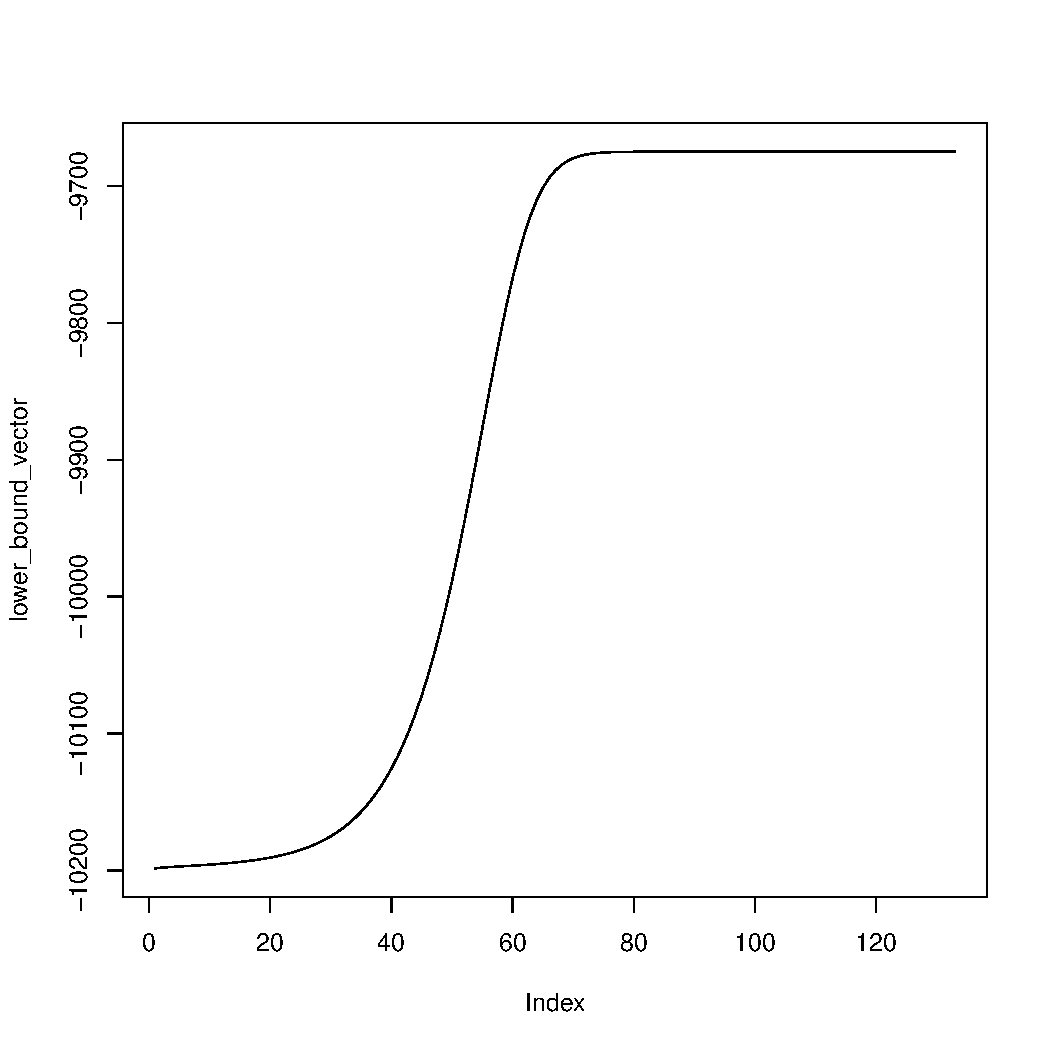
\includegraphics[width=100mm,height=100mm]{code/lower_bound_convergence.pdf}
\end{figure}

% Accuracy results.
% Figures of the MCMC and approximate distributions.


\section{Extending the zero-inflated Poisson model to a regression model}
\noindent The above univariate model demonstrates that variational approximations are well-suited
to accelerating the fit of Bayesian zero-inflated models to data. Typically zero-inflated
models arise in applications where we wish to build multivariate regression models. To be able to
construct multivariate models with as much generality as possible, we specify the full
model as a General Design Bayesian Generalized Linear Mixed Model, as in \citep{zhao06}.
This allows us to incorporate within-subject correlation, measurement error, missing data
and smoothing splines in our models.

% TODO: Lower bound graph
% TODO: Accuracy of approximations
% TODO: Application, physical activity data
% Random intercept, longitudinal data
% Graph demonstrating additional zeroes

% Idea: We can use an approximation of the from q(\beta, \u, \Sigma) q(\rho) \Product q(r_i)
% and use GVA on q(\beta, \u, \Sigma) and mean field updates on \rho and r_i

\subsection{Model}
Let $\mR = \diag{(\vr)}$. Let $\mC = [\mX \mZ], \vnu = [\vbeta^T \vu^T]^T$.

$$
\begin{array}{rl}
\log{p(y|\vr, \vbeta, \vu)} &= \vy^T \mR (\mC\vnu) - \vr^T \exp{(\mC\vnu)} - \vone^T \log{\Gamma{(\vy + \vone)}}, \\
\log{p(\vnu|\sigma_{u}^2)} &= - \half \log{|2\pi \sigma_{\vu}^2 \mI|} - \half \vnu^T(\sigma_{\vu}^2 I)^{-1} \vnu, \\
\log{p(\vr)} &= \vr^T \log{(\rho \vone)} + (\vone - \vr)^T\log{(\vone - \vone \rho)}, \\
p(\rho) &\propto 1, \\
\mbox{and } \log{p(\sigma^2)} &= \alpha_{\sigma_\vu^2} \log{(\beta_{\sigma_\vu^2})} - \log{\Gamma{(\alpha_{\sigma_\vu^2})}} - (\alpha_{\sigma_\vu^2} + 1) \log{(\sigma_{\vu}^2)} - \frac{\beta_{\sigma_\vu^2}}{\sigma_{\vu}^2}\\
\end{array}
$$

\subsection{Approximation}
Let $r_0 = \{ r_i : y_i = 0 \}$.
We assume an approximation of the form
$$
q(r_0, \vnu, \sigma_{\vu}^2, \rho) = q(\vnu) q(\sigma_{\vu}^2) q(\rho) q(r_0) \\
$$

\noindent where

%\begin{align*}
$$
\begin{array}{rl}
q(\vnu) &= \mbox{N}(\vmu, \mLambda), \\
q(\sigma_{\vu}^2) &= \mbox{IG}\left(\alpha_{\sigma_u^2} + \frac{m}{2}, \beta_{\sigma_u^2} + \frac{\|\vmu_\vu\|^2}{2} + \frac{\tr(\mLambda_{\vu\vu})}{2}\right), \\
\mbox{and } q(r_i) &= \Bernoulli{(p_i)}
\end{array}
$$
%\end{align*}

\noindent where
$$
p_i = \expit\left[ \psi{(\alpha_{q(\rho)})} - \psi{(\beta_{q(\rho)})} - \exp{(c_i^T\vmu + \half c_i^T \mLambda c_i)} \right]
$$

\noindent \text{when} $\vy_i = 0$.

% What on Earth is this section doing here? This is very random.
%$\propto \exp{\left \{-r_i \bE_{-r_i} [\exp{(c_i^T\vnu)}] + r_i [\psi(\alpha_\rho) - \psi(\beta_\rho)] \right \} }.\\$

% Include derivations for mean field updates at the end?

\noindent The optimal approximation for $\vr$ is
$$
\begin{array}{rl}
q(\vr) &\propto \exp \left [ \bE_{-q(\vr)}y^T\mR(\mC\vmu) - \vr^T\exp{(\mC\vnu)}-\half \vnu^T \text{diag}(\sigma_{\vu}^2)^{-1} \vnu \right ] \\
&= \exp{\left [\vy^T\mR\mC \vmu - \vp^T \exp{\{\mC \vmu + \half \text{diag}(\mC \mLambda \mC^T)\}} - \half \vmu^T \hat{\mD} \vmu - \half \text{tr}(\mLambda \hat{\mD} )) \right ]}
\end{array}
$$

\noindent where $\hat{\mD} = \text{diag}\left (\alpha_{q(\sigma_{\vu}^2)}/\beta_{q(\sigma_{\vu}^2)} \right )$. 

\noindent This is close in form to a Poisson regression model. Poisson regression models
with normal priors have no closed form for their mean field updates due to
non-conjugacy, but can be fit using Gaussian variational approximation
\citep{ormerod09}. The model can be fit using Algorithm 2 below.

\begin{algorithm}\label{alg:algorithm_two}
\label{algorithm2}
\caption[Algorithm 2]{Iterative scheme for obtaining the parameters in the
optimal densities $q^*(\vmu, \mLambda)$, $q^*(\sigma_u^2)$ and $q^*(\rho)$}
\begin{algorithmic}
% Fit \vmu, \mLambda using Laplace approximation
\REQUIRE{$\alpha_{q(\rho)} \leftarrow \alpha_\rho + \vone^T\vp, 
\alpha_{q(\lambda)} \leftarrow \alpha_\lambda + \vone^T\vx$}
\WHILE{the increase in $\log{\underline{p}}(\vx;q)$ is significant}
% \vmu, \mLambda
\STATE Optimise $\vmu$ and $\mLambda$ using $\vy, \mX, \mZ, \rho, \vp$ and
$\alpha_{q(\sigma_u^2)}$, $\beta_{q(\sigma_u^2)}$
\STATE $\beta_{q(\lambda)} \leftarrow \beta_\lambda + \vone^T\vp$
% \vp
% \rho is a prior? Not directly observed, except through \vr_i
\STATE $\beta_{q(\rho)} \leftarrow \beta_\rho + n - \vone^T\vp$
\STATE $\eta \leftarrow -\exp \left [ \mC \vmu + \half \diag{(\mC\mLambda\mC^T)} \right ] + \psi{(a_{q{(\rho)}})} - \psi{(b_{q{(\rho)}})}$
\STATE $\vp_{q(\vr_0)} \leftarrow \expit{(\eta)}$
% sigma_u^2
\ENDWHILE
\end{algorithmic}
\end{algorithm}


\subsection{Lower bound}
% Where are the priors for \vbeta and \vu
\noindent The lower bound is equal to
$\bE_q[\log{p(\vy, \vtheta)} - \log{q(\vtheta)}] = T_1 + T_2$,
where $T_1$ is as defined below and $T_2$ is the same as in the univariate
model.

% This is the new T_1
$$
\begin{array}{rl}
$T$_1 &= \bE_q[\log{p(\vy, \vnu)} - \log{q(\vnu)}] \\
&= \quad \vy^T \mP \mC \vmu - \vp^T \exp{\left [\mC \vmu + \half \text{diag} (\mC \mLambda \mC^T)\right ]} - \vone^T\log \Gamma{(\vy + \vone)}\\
& \quad + \frac{p + m}{2} (1 + \log{2 \pi}) + \half \log{|\mLambda|},
\end{array}
$$

where $A_q = A + m/2$ and $B_q = B + \|\vmu_\vu\|^2/2 +  \tr{(\mLambda_{\vu \vu})}/2$.

\subsection{Optimising the GVA lower bound}
% Detail techniques used for fitting models.
The Gaussian variational lower bound in Algorithm 2 can be optimised using a 
variety of algorithms. Each of these algorithms is a trade-off between accuracy, 
stability and speed.

\subsubsection{Laplace's method}
Laplace's method of approximation relies on a second order Taylor expansion of the
log likelihood around the mode. This can then be optimised with Newton-Raphson
iterations. The algorithm is very quick to execute, but the resulting approximate
posterior distributions are not as accurate as those produced by the other algorithms
considered in this article.

% NR
% Detail the function and its derivatives
Taylor expanding the variational lower bound once around the mode yields the following function
\begin{align*}
\log \underline{p}(\vmu, \mLambda; \vy) = \vp^T\vy^T\mC\vmu - \vp^T\exp \left (\mC \vmu + \half \mC \mLambda \mC^T \right ) - \half \vmu^T \mSigma^{-1} \vmu - \half \tr{(\mLambda \mSigma^{-1})}
\end{align*}

This can be optimised using a Newton-Raphson style algorithm where

\begin{align*}
\nabla \log \underline{p}(\vmu, \mLambda; \vy) &= \vp^T\mC(\vy - \exp{(\mC \vmu)}) - \mSigma^{-1} \vmu \\
\nabla^2 \log \underline{p}(\vmu, \mLambda; \vy) &= -\mC^T \text{diag}(\exp{(\mC \vmu)}) \mC - \mSigma^{-1}
\end{align*}

\begin{algorithm}\label{alg:algorithm_three}
\caption[Algorithm 3]{Newton-Raphson scheme for optimising $\log \underline{p}(\vmu, \mLambda; \vy)$}
\begin{algorithmic}
% Fit \vmu, \mLambda using Laplace approximation
\WHILE{the increase in $\log \underline{p}(\vmu, \mLambda; \vy)$ is significant}
% \vmu, \mLambda
\STATE $\mLambda \leftarrow \left [\mC^T \text{diag}(\exp{(\mC \vmu)}) \mC + \mSigma^{-1} \right ]^{-1}$
\STATE $\vmu \leftarrow \vmu + \mLambda \nabla \log \underline{p}(\vmu, \mLambda; \vy)$
\ENDWHILE
\end{algorithmic}
\end{algorithm}

\subsubsection{GVA}
% More complicated functions and derivatives, but more accurate
The first variant of the Gaussian Variational Approximation algorithm
optimises the Gaussian variational lower bound of the log likelihood with respect
to $\vmu$ and the Cholesky decomposition $\mR$ of $\mLambda$, that is,
$\mLambda = \mR \mR^T$. This algorithm trades the computational complexity of 
numerically evaluating the integral in Equation \ref{eq:gva} for greatly increased 
accuracy in the approximating posterior distribution.

The resulting function is below and can be optimised with L-BFGS:

% Detail the function and its derivatives
\begin{align}\label{eq:gva}
\log \underline{p}(\vmu, \mLambda; \vy) &= \vp^T\vy^T\mC \vmu - \vp^T \B(\mC \vmu, \text{diag}(\mC \mLambda \mC^T)) - \half \vmu \mSigma^{-1} \vmu - \half \tr{(\mSigma^{-1} \mLambda)} \\
&\quad - \frac{d}{2} \log{(2 \pi)} + \half \log{|\mSigma^{-1}|} + \frac{d}{2} \log{(2 \pi)} + \frac{d}{2} + \log{|\mR|}
\end{align}

\begin{align*}
\nabla \log \underline{p}(\vmu, \mLambda; \vy) &= \mC^T \vp^T(\vy - \B^{(1)}(\mC \vmu, \mC \mLambda \mC^T)) - \mSigma^{-1}
\end{align*}

\begin{align*}
\nabla^2 \log \underline{p}(\vmu, \mLambda; \vy) &= [\mLambda^{-1} - \vp^T \mC^T \text{diag}(\B^{(2)}(\mC \vmu, \mC \mLambda \mC^T)) \mC \vp) - \mSigma^{-1}] \mR
\end{align*} 
 
\subsubsection{GVA2}
The second variant of the Gaussian Variational Approximation algorithm is similiar to
the first, but instead of optimising $\vmu$ and $\mR$ where $\mLambda=\mR \mR^T$,
instead we optimise $\mR$ where $\mLambda = (\mR \mR^T)^{-1}$.
% The function and derivatives change
This has the advantage that if we re-order the columns of $\mLambda$ such that
the random effects are placed before the fixed effects then due to the assumed 
independence between the random effects, the off-diagonals of the Cholesky decomposition
will 0s and so the Cholesky factor $\mR$ will be sparse. This mitigates the increased
computational complexity of this algorithm versus Laplace's method to some degree.

% More complicated functions and derivatives, but more accurate
% Can be quite fast because of the special form of $\mR$.

% Detail the function and its derivatives under this parameterisation
% Difficulties re: multimodal likelihood, tricks to get that to work
The variational lower bound is not necessarily unimodal, leading to potential
difficulty in optimising to the global maximum. This problem was sidestepped by
optimising the parameter estimates using Laplace's method first to get a rough
estimate, then using the GVA2 algorithm to further refine that estimate. This led
to an extremely accurate approximation of the true posterior at the expense of some
additional computational effort.
% Re-order the covariance matrix so that Chevron form is ``reversed''. This makes
% the Cholesky factorisation very simple, and reduces the number of parameters that
% you need to optimise and store.

\begin{align*}
\log \underline{p}(\vmu, \mLambda; \vy) &= \vp^T\vy^T\mC \vmu - \vp^T \B(\mC \vmu, \text{diag}(\mC \mLambda \mC^T)) - \half \vmu \mSigma^{-1} \vmu - \half \tr{(\mSigma^{-1} \mLambda)} \\
&\quad- \frac{d}{2} \log{(2 \pi)} + \half \log{|\mSigma^{-1}|} + \frac{d}{2} \log{(2 \pi)} + \frac{d}{2} - \log{|\mR|}
\end{align*}

The first derivative is the same as that in the GVA algorithm, but as the parameterisation of
$\mLambda$ has changed, the second derivative is now

\begin{align*}
\nabla^2 \log \underline{p}(\vmu, \mLambda; \vy) &= -\mR^{-1}\left [\mLambda^{-1} - \vp^T \mC^T \text{diag}(\B^{(2)}(\mC \vmu, \mC \mLambda \mC^T)) \mC \vp - \mSigma^{-1} \right ]\mLambda
\end{align*} 

\subsubsection{GVA NR}
This variant of the algorithm uses Newton-Raphson optimisation on the Gaussian
variational lower bound. This algorithm is fast, but potentially unstable.
% Essentially a very straightforward optimisation approach, but potentially unstable.
% Detail the function and its derivatives
\begin{align*}
\nabla \log \underline{p}(\vmu, \mLambda; \vy) &= \mC^T\vp \left [\vy - \B^{1}(\mC \vmu, \text{diag}(\mC \mLambda \mC^T)) \right ] - \mSigma^{-1} \vmu
\end{align*}

\begin{align*}
\nabla^2 \log \underline{p}(\vmu, \mLambda; \vy) &= -\mC^T \text{diag}(\vp \odot \B^{(2)}(\mC \vmu, \text{diag}(\mC \mLambda \mC^T))) - \mSigma^{-1}
\end{align*}

\begin{algorithm}\label{alg:algorithm_nr}
\label{algorithm_nr}
\caption[Algorithm GVA NR]{Iterative scheme for obtaining optimal $\vmu$ and $\mLambda$
given $\vy$, $\mC$ and $\vp$}
\begin{algorithmic}
% Fit \vmu, \mLambda using Laplace approximation
\WHILE{the increase in $\log{\underline{p}}(\vmu, \mLambda; \vy)$ is significant}
% \vmu, \mLambda
\STATE $\mLambda \leftarrow (\mC^T\vp^T B^{(2)}(\mC \vmu, \text{diag}(\mC \mLambda \mC^T)) \mC)^{-1}$
\STATE $\vmu \leftarrow \vmu + \mLambda \nabla \log \underline{p}(\vmu, \mLambda; \vy)$
\ENDWHILE
\end{algorithmic}
\end{algorithm}

% Splines

\subsection{Results/Numerical experiments}\label{sec:results}

% Comparison with MCMC
Our approximation algorithms were compared with the posterior distribution estimated
by kernel density estimate from a 1 million MCMC sample produced using Stan.
% It works
% Stability was confirmed over 100 randomly generated data sets.

The stability of the algorithms was confirmed by running them on 100 different
data sets that were randomly generated after having initialised the random number
generator with different seeds.

% Table of accuracy results
% Graphs - exactly what sort of graphs do we need?
% Increase in lower bound
% MCMC posterior, with approximating posterior for at least one or two of the
% key parameters, such as, say, vbeta[2]


\section{Application}\label{sec:application}

% This section can probably be dropped.
\section{Theory of variational approximation of zero-inflated Poisson models}
Let $Z_i = R_i Y_i$.

Then the probability that $Z_i = 0$ is
$$
\begin{array}{rl}
P(Z_i = 0) &= P(R_i = 0)P(Y_i = y) + P(R_i = 1) P(Y_i = 0) - P(R_i = 0) P(Y_i = 0) \\
&= (1 - \rho) + \rho e^{-\lambda} - (1 - \rho) e^{-\lambda} \\
&= (1 - \rho) + e^{-\lambda}(2 \rho - 1)
\end{array}
$$

\section{Appendix} 

\subsection{Mean field update equations}
We are now in a position to calculate the mean field update equations for the factorised
variational approximation.
Assuming that $q(r_i) \sim \Bernoulli{(p_i)}$ then,

% Mean field update for q(\lambda)
$$
\begin{array}{rl}
q^*(\lambda)
    & \propto 
    \lambda^{\alpha_\lambda+\vone^T\vx - 1} 
    \exp\left\{ 
    \bE_{-q(\lambda)} \left[
    -(\beta_\lambda + \vone^T\vr) \lambda 
    \right] 
    \right\} 
    \\ [0.5ex]
    &
    \propto \lambda^{\alpha_\lambda+\vone^T\vx - 1} \exp{\left \{-(\beta_\lambda + \vone^T\vp)\lambda \right \} } 
\\
    & = \myGamma{(\alpha_\lambda+\vone^T\vx, \beta_\lambda+\vone^T\vp)},
\end{array}
$$

% Mean field update for q(\rho)
$$
\begin{array}{rl}
\log{q^*(\rho)} 
    &
    \propto \left\{ 
    \bE_{-q(\rho)}\left[ 
    \vone^T\vr \log{(\rho)} 
    + (n - \vone^T\vr) \log{(1 - \rho)} 
    \right] 
    + \alpha_\rho \log{(\rho)} 
    + \beta_\rho \log{(1 - \rho)} 
    \right\} 
    \\ [0.5ex]
    &
    \propto \exp \left( 
    (\vone^T\vp + \alpha_\rho) \log{(\rho)} 
    + (n - \vone^T\vp + \beta_\rho) \log{(1 - \rho)} 
    \right) 
    \\ [0.5ex]
    &= \Beta(\alpha_\rho + \vone^T\vp, \beta_\rho + n - \vone^T\vp),
\end{array}
$$

\noindent and

$$
\begin{array}{rl}
\ds \log{q^*(r_i)} &\propto -\bE_{q(\lambda)} [\lambda ] r_i + x_i \log{(r_i)} + r_i \bE_{q(\rho)} \left[\log{\left(\frac{\rho}{1 - \rho}\right)}\right]\\[0.5ex]
& \ds = -r_i \frac{\alpha_{q(\lambda)}}{\beta_{q(\lambda)}} + x_i \log{(r_i)} + r_i \left(\psi(\alpha_{q(\rho)}) - \psi(\beta_{q(\rho)})\right)\\ [0.5ex]%
& \ds = \text{Bernoulli}(p_i)
\end{array}
$$

\noindent where

$$
\begin{array}{rl}
\ds p_i 
     = \frac{\exp{(\eta_i)}}{I(x_i = 0) + \exp{(\eta_i)}}  
     = \text{expit}(\eta_i), \quad \mbox{(when $x_i = 0$)} 
\end{array}
$$

\noindent and $\eta_i = - \alpha_{q(\lambda)}/\beta_{q(\lambda)} + \psi(\alpha_{q(\rho)}) - \psi(\beta_{q(\rho)})$.

\noindent The optimal approximation for $\vr$ is
$$
\begin{array}{rl}
q(\vr) &\propto \exp{\{\bE_{-q(\vr)}y^T\mR(\mC\vmu) - \vr^T\exp{(\mC\vnu)}-\half \vnu^T \text{diag}(\sigma_{\vu}^2)^{-1} \vnu\}}
\end{array}
$$

$$
\begin{array}{rl}
&\bE_{-q(\vr)} [\vy^T\mR(C\vnu) - \vr^T\exp{(\mC\vnu)}-\half \vnu^T \text{diag}(\sigma_{\vu}^2)^{-1} \vnu]\\
=&\vy^T\mR\mC \vmu - \vp^T \exp{\{\mC \vmu + \half \text{diag}(\mC \mLambda \mC^T)\}} - \half \vmu^T \hat{\mD} \vmu - \half \text{tr}(\mLambda \hat{\mD} ))
\end{array}
$$

\subsection{Lower bound}
The lower bound $\log{\underline{p}(\vtheta)}$ is
$$
	\bE_q[\log{p(\vx, \vtheta)} - \log{q(\vtheta)}]
$$

\noindent where $q(\vtheta) = q(\lambda) q(\rho) \prod_{i=1}^n q(r_i)$,
$q(\lambda) \sim \text{Gamma}{(\alpha_{q(\lambda)}, \beta_{q(\lambda)})}$,
$q(\rho) \sim \text{Beta}(\alpha_{q(\rho)}, \beta_{q(\rho)})$ and
$q(r_i) = 1$ if $x_i \ne 0$, and $p_i$ if $x_i = 0$, where $p_i$ is
calculated for each iteration as specified in Algorithm \ref{algorithm1}.

The lower bound can be calculated directly to be
$$
\begin{array}{rl}
\bE_q \left\{ \log{p(\vx, \vr, \lambda, \rho)} - \log{q(\vr, \lambda, \rho)} \right\} &= T_1 + T_2 \\
\end{array}
$$

\noindent where
$$
\begin{array}{rl}
T_1 & \ds =
\alpha_\lambda \log{(\beta_\lambda)} + (\alpha_\lambda - 1) \bE_q[\log{(\lambda)}] - \beta_\lambda \bE_q [\lambda] - \log\Gamma(\alpha_\lambda) \\
& \ds \quad + \sum_{i=1}^n ( -\bE_q [\lambda] \bE_q [r_i] + \bE_q[x_i \log{(\lambda r_i)}] - \log\Gamma(x_i+1)) \quad \mbox{and}
\\ [1ex]
T_2 &=\bE_q[r_i] \bE_q[\log{(\rho)}] + \bE_q[(1 - r_i)] \bE_q[\log{(1 - \rho)}] 
- \bE_q[\log{q(r)}] 
- \bE_q[\log{q(\lambda)}] 
- \bE_q[ \log{q(\rho)}]
\end{array}
$$

\noindent with 
$\bE[\lambda] = \alpha_{q(\lambda)}/\beta_{q(\lambda)}$,
$\bE [\lambda] = \alpha_{q(\lambda)}/\beta_{q(\lambda)}$,
% T_1 terms
$$
\begin{array}{rl}
\bE [\log{\lambda}] & \ds = -\{ \alpha_{q(\lambda)} - \log{(\beta_{q(\lambda)})} + \log{\Gamma(\alpha_{q(\lambda)})} + (1 - \alpha_{q(\lambda)}) \psi{(\alpha_{q(\lambda)})} \}, \\
 \\
\bE[\log{\rho}] & \ds = - \{ \log{\text{Beta}(\alpha_{q(\rho)}, \beta_{q(\rho)})} - (\alpha_{q(\rho)} - 1) \psi{(\alpha_{q(\rho)})} - (\beta_{q(\rho)} - 1)\psi{(\beta_{q(\rho)})} \\
    & \ds \qquad + (\alpha_{q(\rho)} + \beta_{q(\rho)} - 2)\psi{(\alpha_{q(\rho)} + \beta_{q(\rho)})} \},
\\
\bE[r_i] & \ds = 
	\begin{cases}
	1 & \text{if } x_i \ne 0 \\
	p_i & \text{if } x_i = 0, \\
	\end{cases}
\\
-\bE_q[\log{q(r)}] & \ds = \sum_{i=1}^n I(x_i = 0) \log{(p_i)} \\ [0.5ex]
-\bE_q[\log{q(\lambda)}] 
    & \ds = \alpha_{q(\lambda)} - \log{(\beta_{q(\lambda)})} + \log{\Gamma{(\alpha_{q(\lambda)})}} + (1 - \alpha_{q(\lambda)}) \psi{(\alpha_{q(\lambda)})}, \\ [0.5ex]
 \mbox{and}\quad \bE_q[\log{q(\rho)}] 
    & \ds = - \{ \log{(\text{Beta}(\alpha_{q(\rho)}, \beta_{q(\rho)})} - (\alpha_{q(\rho)} - 1) \psi{(\alpha_{q(\rho)})} - (\beta_{q(\rho)} - 1)\psi{(\beta_{q(\rho)})}  \\ [0.5ex]
& \ds \quad + (\alpha_{q(\rho)} + \beta_{q(\rho)} - 2)\psi{(\alpha_{q(\rho)} + \beta_{q(\rho)})} \}. \\ [0.5ex]
\end{array}
$$

\section{Appendix - Algebraic derivations of conditional likelihoods}

The joint likelihood is:

$$
p(\vx, \vr, \lambda, \rho) = \frac{b^a \lambda^{a - 1} \exp{(-b \lambda)}}{\Gamma{(a)}} \prod_{i=1}^n \frac{\exp{(-\lambda r_i)} (\lambda r_i)^{x_i}}{x_i !} \rho^{r_i} (1 - \rho)^{1 - r_i}.
$$

%\begin{align*}
%p(\lambda|\vx, \vr, \rho) &= \frac{\prod_{i=1}^n p(x_i | \lambda, r_i) p(\lambda) p(r_i|\rho) p(\rho)}{\int \prod_{i=1}^n p(x_i | \lambda, r_i) p(\lambda) p(r_i|\rho) p(\rho)) d \lambda}.
%\end{align*}
%
%Concentrating for now on the denominator in this expression, we re-arrange and collect
%like terms to obtain
%$$
%\prod_{i=1}^n \rho^r_i (1 - \rho)^{1 - r_i} \frac{r_i^{x_i}}{x_i !}
%	\int \frac{b^a \lambda^{a - 1} \exp{(-b \lambda)} \lambda^{x_i} \exp{(-\lambda r_i)}}{\Gamma{(a)}} d \lambda
%$$
%
%The integral in this expression is
%\begin{align*}
%& \int \frac{b^a \lambda^{(a + x_i) - 1} \exp{(-\lambda(b + r_i))}}{\Gamma{(a + x_i)}} d \lambda \frac{\Gamma{(a+ x_i)}}{\Gamma{(a)} b^{-x_i}} \\
%=& \frac{\Gamma{(a+ x_i)}}{\Gamma{(a)} b^{-x_i}}.
%\end{align*}
%
%Collecting the multiplicands in the integral over $\lambda$ together, we obtain
%$$
%\prod_{i=1}^n \rho^{r_i} (1 - \rho)^{1 - r_i} \frac{r_i^{x_i}}{x_i!}
%	\int \frac{b^{na + \sum_{i=1}^n x_i} \lambda^{(na + \sum_{i=1}^n x_i) - 1} \exp{(-\lambda(nb + \sum_{i=1}^n r_i))}}{\Gamma{(na + \sum_{i=1}^n x_i)}} d \lambda
%	\frac{\Gamma{(na + \sum_{i=1}^n x_i)}}{\Gamma{(na)} b^{-\sum_{i=1}^n x_i}}.
%$$

%By cancelling like terms in the numerator and denominator of the full likelihood we arrive 
%at

$$
\beta_{\lambda}^{\alpha_\lambda+\vone^T\vx} \lambda^{(\alpha_\lambda + \vone^T\vx) - 1} \exp{\left(-(\beta_\lambda + \vone^T\vr) \lambda \right)}
$$

$$
\frac{\rho^{\vone^T\vr} (1 - \rho)^{\vone^T(\vone - \vr)}}{\Beta{\alpha_\rho + \vone^T \vr, \beta_\rho + \vone^T(\vone - \vr)}}
$$

$$
\begin{array}{ll}
p(r_i | \text{rest}) & \ds \propto \frac{(\lambda r_i)^{x_i} \exp{(-\lambda r_i)}}{x_i !} \rho^{r_i} (1 - \rho)^{1 - r_i} \\
& \ds \propto r_i^{x_i} (e^{-\lambda})^{r_i} \rho^{r_i} (1 - \rho)^{1 - r_i}
\end{array}
$$

We make use of the fact that if $x_i = 0$, $r_i = 0$, and if $x_i \ne 0$,
$r_i = 1$. So $x_i^{r_i} = I(x \ne 0)$ and hence the likelihood can be re-written as

$$
\begin{array}{ll}
p(r_i | \text{rest}) & \ds = \frac{(e^{-\lambda + \logit{(\rho)}})^{r_i}}{I(x_i = 0) + (e^{-\lambda + \logit{(\rho)}})^{r_i}}
\end{array}
$$

\bibliographystyle{elsarticle-harv}
\bibliography{Chapter_1_zero_inflated_models}

\end{document}
